\documentclass[UTF8, heading=true]{ctexart}
\usepackage{karnaugh-map}
%-----中文宏包-----
\usepackage[UTF8]{ctex}
\usepackage[utf8]{inputenc}
\usepackage{titling}
%-----数学宏包-----
\usepackage{amsmath,amsthm,amssymb,amsfonts}
\usepackage{mathrsfs,bm}
\usepackage{dirtree}
%-----draft下 label提示-----
%\usepackage[notcite,notref]{showkeys}
%-----页面布局-----
\usepackage{geometry}
\geometry{left=1.25in,right=1.25in,top=1in,bottom=1in}
%\geometry{left=1in,right=1in,top=1in,bottom=1in}
%\geometry{left=2.5cm,right=2.1cm,top=1.7cm,bottom=2cm,includehead,includefoot}

%-----设置超链接-----
\usepackage{url,hyperref}
\hypersetup{colorlinks=true,linkcolor=black,citecolor=black} % 去掉目录红框
%-----制作目录-----
\usepackage{imakeidx}
% 设置颜色
% \usepackage{color,xcolor}
% 插入图片
\usepackage{graphicx}
\usepackage{epsfig}
%-----设置表格-----
\usepackage{tabularx,array}
\usepackage{longtable}
\usepackage{booktabs}
\usepackage{multirow}
\usepackage{multicol}
\usepackage{fancybox}
%-----调整单元格格式-----
\usepackage{makecell}
%-----操作字符串-----
\usepackage{xstring}
%-----设置章节标题和目录-----
\usepackage{titletoc}
\usepackage{titlesec}
%-----数学公式扩展-----
\usepackage{mathtools}
%-----浮动体设置-----
\usepackage{float}
%-----书签设置-----
\usepackage{bookmark}
%-----参考文献格式-----
\usepackage[numbers]{natbib}
%-----设置页眉页脚格式-----
\usepackage{fancyhdr}
% --- 设置代码环境 -----
\usepackage{color,xcolor}
\usepackage{listings}
\definecolor{bg}{rgb}{0.95, 0.95, 0.95}
\definecolor{keywordcolor}{rgb}{0.0, 0.0, 0.5}
\definecolor{commentcolor}{rgb}{0.0, 0.5, 0.0}
\definecolor{stringcolor}{rgb}{0.6, 0.1, 0.0}

% 设置 listings 样式
\lstdefinestyle{cppstyle}{
    language=C++,
    backgroundcolor=\color{bg},
    basicstyle=\small\ttfamily,
    keywordstyle=\color{keywordcolor}\bfseries,
    commentstyle=\color{commentcolor}\itshape,
    stringstyle=\color{stringcolor},
    numbers=left,
    numberstyle=\tiny\color{gray},
    numbersep=5pt,
    frame=lines,
    breaklines=true,
    breakatwhitespace=false,
    tabsize=4,
    showtabs=false,
    showspaces=false,
    showstringspaces=false,
    captionpos=b,
    keepspaces=true,
    columns=flexible,
    xleftmargin=2em,
    framexleftmargin=1.5em,
    framexrightmargin=0.5em,
    framesep=2mm,
    escapeinside={(*@}{@*)},
    morekeywords={glm, VertexData, Vector3f, Vector4f, Eigen, auto}
}

\lstdefinestyle{pythonstyle}{
    language=Python,
    backgroundcolor=\color{bg},
    basicstyle=\small\ttfamily,
    keywordstyle=\color{keywordcolor}\bfseries,
    commentstyle=\color{commentcolor}\itshape,
    stringstyle=\color{stringcolor},
    numbers=left,
    numberstyle=\tiny\color{gray},
    numbersep=5pt,
    frame=lines,
    breaklines=true,
    breakatwhitespace=false,
    tabsize=4,
    showtabs=false,
    showspaces=false,
    showstringspaces=false,
    captionpos=b,
    keepspaces=true,
    columns=flexible,
    xleftmargin=2em,
    framexleftmargin=1.5em,
    framexrightmargin=0.5em,
    framesep=2mm,
    escapeinside={(*@}{@*)},
    morekeywords={import, from, def, class, if, else, for, while, return}
}

\lstset{style=cppstyle}

% ---- 定义列表项的样式 -----
\usepackage{enumitem}
\setlist{nolistsep}
% --- 设置英文字体 -----
\usepackage{fontspec}
\setmainfont{Times New Roman}
% 指定中文主字体，避免中文缺字问题（Windows 常见为 SimSun/宋体）
\setCJKmainfont{SimSun}
\usepackage{setspace}

\geometry{
  left=3.0cm,        % 左边距
  right=3.0cm,       % 右边距
  top=2.5cm,         % 上边距
  bottom=2.0cm       % 下边距
}
\renewcommand*{\baselinestretch}{1.5}
\newcommand{\upcite}[1]{\textsuperscript{\textsuperscript{\cite{#1}}}}

\renewcommand{\thesection}{\chinese{section}、}
\renewcommand{\thesubsection}{（\chinese{subsection}）}
\renewcommand{\thesubsubsection}{\arabic{subsubsection}.}
\titleformat{\section}{\bfseries \zihao{-3}}{\chinese{section}、}{0em}{}
\titleformat{\subsection}{\bfseries \zihao{4}}{（\chinese{subsection}）}{0.2em}{}
\titleformat{\subsubsection}{\bfseries \zihao{-4}}{\arabic{subsubsection}、}{0.2em}{}
\newcommand{\stunum}[1]{\def\defstunum{#1}}
\newcommand{\class}[1]{\def\defclass{#1}}

% ----- 设置浮动体间距 ------
\setlength{\textfloatsep}{0pt}
\setlength{\floatsep}{10pt plus 3pt minus 2pt}
\setlength{\intextsep}{10pt}
\setlength{\abovecaptionskip}{2pt plus1pt minus1pt}
\setlength{\belowcaptionskip}{3pt plus1pt minus2pt}

% ----- 设置公式间距为零 ------
\AtBeginDocument{
	\setlength{\abovedisplayskip}{4pt plus1pt minus1pt}
	\setlength{\belowdisplayskip}{4pt plus1pt minus1pt}
	\setlength{\abovedisplayshortskip}{2pt}
	\setlength{\belowdisplayshortskip}{2pt}
	\setlength{\arraycolsep}{2pt}   % array中列之间空白长度
}



% --- 自定义命令 -----
\newcommand{\CC}{\ensuremath{\mathbb{C}}}
\newcommand{\RR}{\ensuremath{\mathbb{R}}}
\newcommand{\A}{\mathcal{A}}
\newcommand{\ii}{\bm{\mathrm{i}}\,}  % 虚部
\newcommand{\md}{\mathrm{d}\,}
\newcommand{\bA}{\boldsymbol{A}}
\newcommand{\red}[1]{\textcolor{red}{#1}}
\graphicspath{{./img/}}

\pagestyle{fancy}
\fancyhf{}
\fancyfoot[C]{\thepage}
\fancyhead[L]{多模态开题报告}
\fancyhead[R]{文档理解+多模态检索问答系统}
\title{\LARGE \textbf{多模态开题报告 \hspace{0.2cm} 文档理解+多模态检索问答系统}}
\date{}
\author{小组成员1：庄仕豪 \qquad 学号：23336355 \\ 小组成员2: 钟晨辉 \qquad 学号：23336336}

\begin{document}
\maketitle
\vspace{-1.5cm}

\section{任务定义与项目背景}

\subsection{任务定义}

本项目的核心任务是构建一个"文档智能助手"。系统需接收包含复杂排版的视觉密集型输入（如多页PDF、扫描文档、带有图表的讲义截图等），自动完成页面中纯文本、复杂数据表格及图像元素的精确结构化定位与提取。最终，系统能够基于用户的自然语言查询（如"图3的折线表示了什么趋势？"），输出精准的结构化回答，并要求在回答中进行精准的依据溯源，标出引用的具体页面编号或图表序号。

\subsection{应用场景与技术痛点}

在现代企业、金融及科研场景中，高价值知识被长期封存在具有高度复杂排版的PDF文档、包含大量嵌套表格的商业财报、夹杂精密仪器的工业手册及双栏排版的学术论文中\upcite{1}。传统基于纯文本的检索增强生成（Text-RAG）在处理这类文档时，几乎完全依赖光学字符识别（OCR）。这种强制序列化的降维转换，在遇到多栏排版时极易产生跨栏拼接的语义乱码；更为致命的是，它会完全丢失文档中图表走势、图像特征等纯视觉信息，导致大语言模型在回答依赖视觉证据的问题时，由于缺乏上下文而产生严重幻觉。因此，构建保留原始空间与视觉信息的多模态RAG（MM-RAG）系统是突破当前文档问答瓶颈的关键。

\subsection{项目建设目标}

\begin{enumerate}
    \item 构建支持图文联合提取、能够物理隔离存储文本与图像特征的自动化文档预处理流水线。
    \item 深度对比评估"纯文本RAG"与"多模态RAG"在处理复杂文档时的实际召回与推理效果差异。
    \item 实现带依据强溯源的问答生成机制，提高大模型在严肃场景下的忠实度。
    \item 适配普通消费级设备：在普通的 8GB 显存设备上完成文档解析与轻量级特征编码，同时协同云端多模态大模型 API 完成重度推理生成，实现高效部署。
\end{enumerate}

\section{相关工作调研与核心组件选型}

为了确保本系统的设计具有严谨的学术依据与前沿视野，我们对 2024-2025 年文档理解与多模态 RAG 领域的代表性文献、开源项目以及 Embedding 模型进行了调研，这些工作直接指导了本项目的架构设计。

\subsection{代表性文献与开源项目调研}

\begin{enumerate}
    \item \textbf{文档解析基石：IBM Docling (2024)\upcite{2}}

    \begin{itemize}
        \item \textbf{架构与结论}：Docling 摒弃了传统的纯 OCR 路线，内置了基于计算机视觉的 Heron 版面分析模型，能够像人类视觉一样智能识别多栏排版阅读顺序和复杂的表头层级，将其无损转换为结构化 Markdown。
        \item \textbf{对本项目的帮助}：它为我们提供了完美的预处理底层引擎。利用它，我们能够安全地剥离出文档中的表格与图片，并在保留空间拓扑元数据的前提下，建立高质量的纯文本对比基线，彻底解决了传统解析器导致的数据脏乱问题。
    \end{itemize}

    \item \textbf{纯视觉检索天花板：ColPali (ICLR 2025)\upcite{3}}

    \begin{itemize}
        \item \textbf{架构与结论}：该论文提出使用视觉语言模型（PaliGemma-3B），将整张 PDF 页面划分为 1024 个图像网格（Patches），利用后期交互机制（Late Interaction）直接在像素层面对比 Query 与图像的相似度，完全去除了 OCR 环节。
        \item \textbf{对本项目的帮助}：ColPali 证明了"保留原生视觉特征能极大提升检索准确率"这一理论。但同时，其每页产生 1024 个 128 维向量的庞大存储压力与高昂的计算开销，也让我们明确认识到：在普通 8GB 显存设备的约束下，这种直接的密集视觉矩阵计算是不可行的，从而促使我们转向更轻量的多向量摘要路由方案。
    \end{itemize}

    \item \textbf{多文档逻辑编排：M3DocRAG (Preprint 2024)\upcite{6}}

    \begin{itemize}
        \item \textbf{架构与结论}：该研究提出了"三段式"框架：先提取页面视觉特征，再通过近似最近邻（ANN）引擎检索出 Top-K 页面，最后将这几个页面的特征与 Query 统一送入多模态大模型进行跨页推理。
        \item \textbf{对本项目的帮助}：它为我们系统的整体宏观架构提供了直接模板，验证了"检索器（缩小范围）+ 生成器（深度推理）"解耦架构在长篇多模态文档处理中的绝对必要性与有效性。
    \end{itemize}

    \item \textbf{视觉保留的必要性证明：VisRAG (ICLR 2025)}

    \begin{itemize}
        \item \textbf{架构与结论}：论文系统性评估了直接将文档作为图片喂给 VLM 与传统转文本方案的差异。实验数据表明，保留原生排版的端到端生成，能带来 20\% 至 40\% 的综合性能提升。
        \item \textbf{对本项目的帮助}：其结论坚定了我们在生成阶段必须向大模型传入"原始高清图片"而非仅仅是文本描述的决心，这是我们设计后续"代理召回机制"的核心驱动力。
    \end{itemize}

    \item \textbf{融合机制挑战：Ask in Any Modality Survey (2025)}

    \begin{itemize}
        \item \textbf{架构与结论}：该综述全面分析了多模态 RAG 的不同融合策略，指出目前将图像和文本强行映射到同一向量空间的"统一嵌入（Unified Embedding）"往往会遭遇严重的语义对齐鸿沟，导致效果极其不稳定。
        \item \textbf{对本项目的帮助}：这一结论帮助我们排除了高风险的统一向量空间映射方案，指导我们选择了工程上更成熟的"模态文本化（生成摘要）统一检索"的安全路径。
    \end{itemize}
\end{enumerate}


\subsection{Embedding 模型调研与选型}

向量嵌入模型（Embedding Model）是 RAG 系统命中率的命脉。针对 8GB 显存的硬件限制，我们放弃了超大规模模型，重点调研了当前开源生态中体积小巧但性能卓越的文本嵌入模型。

\begin{itemize}
    \item \textbf{BGE-M3 (BAAI, 2024)}：参数量仅 569M，物理体积约 2.27 GB。该模型创新性地支持最高 8192 Tokens 的超长上下文，并且在单一模型内同时支持密集检索（Dense）、稀疏检索（Sparse/BM25）与多向量检索。
\end{itemize}

\textbf{选型结论}：在 CUAD 等专业文档评测基准中，BGE-M3 的表现超越了许多体积大几倍的其他大厂模型。它不仅能以极低的显存占用在本地流畅运行，其超长上下文能力也非常适合对 Docling 提取出的整段复杂表格结构进行不截断的完整语义编码。因此，本系统指定 BGE-M3 为向量化核心组件。

\section{系统总体架构与多模态实现方案设计}

\subsection{多模态 RAG 实现路线分析与选型}

多模态 RAG 的核心难点在于数据库如何同时理解文本与图像。通过调研，当前主要有三种实现方案：

\begin{itemize}
    \item \textbf{方案一}：多模态统一 Embedding。直接使用类似 CLIP 的模型将图文映射到同一空间。优点是结构简单；缺点是图文语义对齐极难，且容易忽略微小的数值文本，效果最不稳定。
    \item \textbf{方案二}：分模态独立 Embedding 加权融合。文本和图片分别建立向量库，查询时计算双路得分并加权。缺点是权重的超参数极难调节，跨模态检索效果差。
    \item \textbf{方案三}：文本主导的多向量检索（Multi-Vector Retriever）。预先利用多模态大模型为图片/表格生成"文本摘要"，统一走文本 Embedding 入库；查询时命中摘要，但最终召回给模型的是原始图片/表格。
\end{itemize}

\textbf{最终选型}：结合前置调研工作得到的信息与本地 8GB 显存的算力硬约束，本项目采用\textbf{方案三}（文本主导的多向量检索）。该方案极大地降低了本地向量检索的算力压力，不仅工程落地极其成熟，还能在最终生成阶段完美保留原始高清图片的视觉特征，是目前性价比与成功率最高的路线。

\subsection{初始系统架构设计}

基于上述路线，系统设计为"本地轻量解析检索 + 云端多模态推理"的协同架构，包含以下四个核心环节：

\begin{figure}[H]
    \centering
    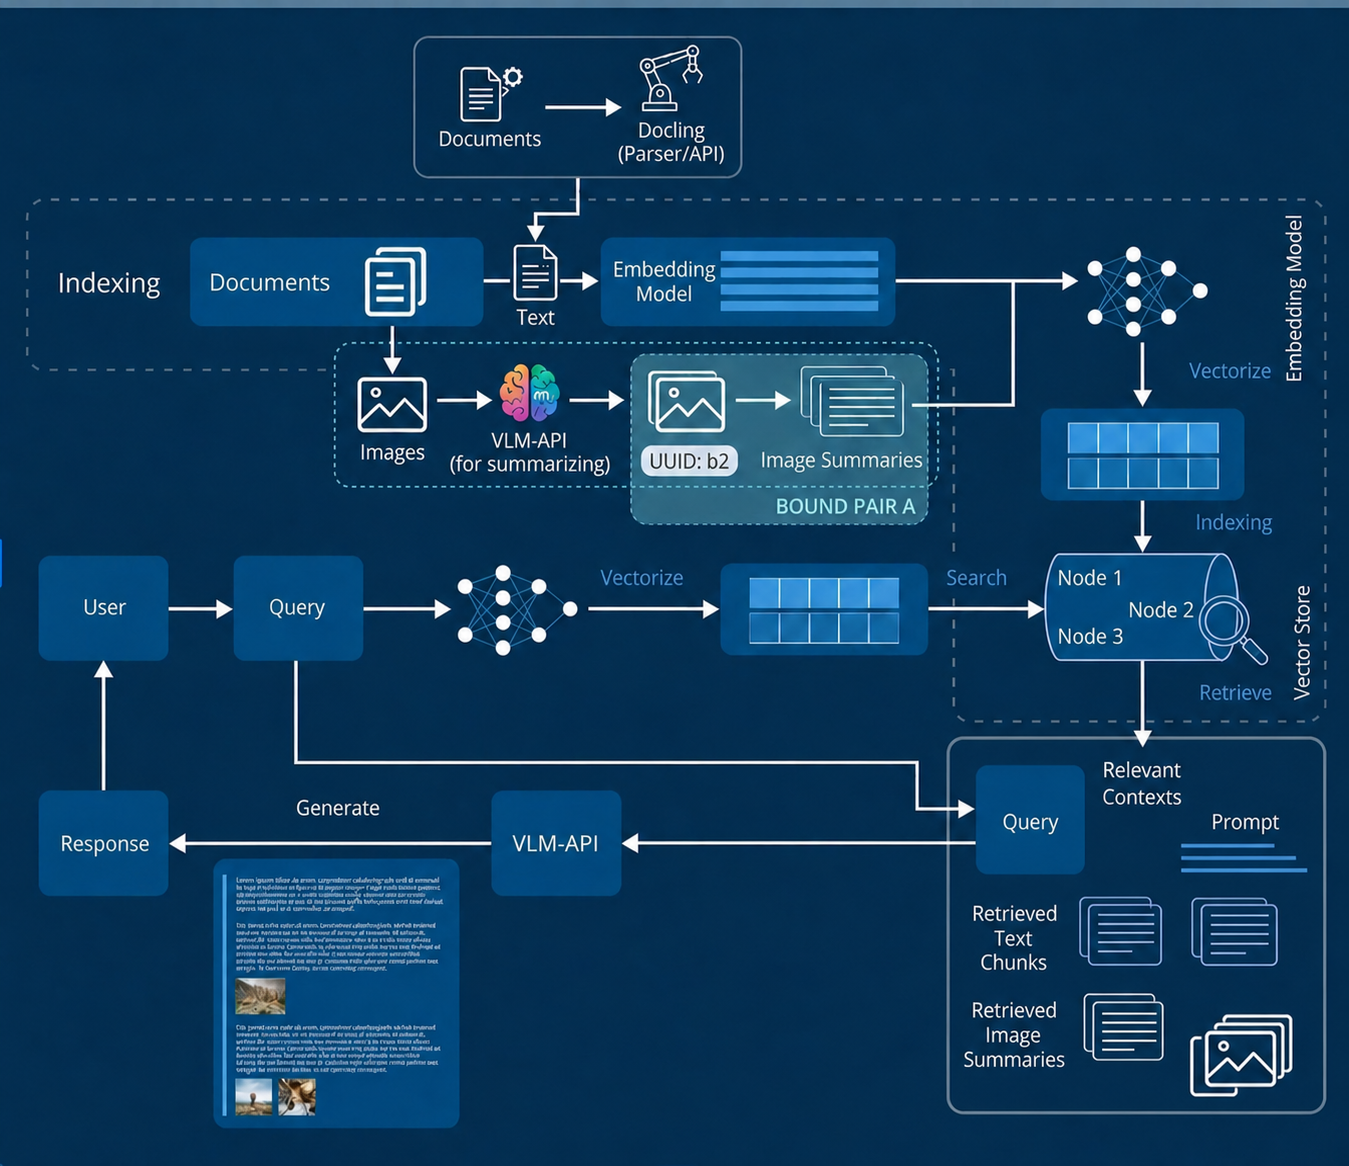
\includegraphics[width=0.9\textwidth]{系统流程图.png}
    \caption{系统总体架构设计图}
\end{figure}

\textbf{1. 文档摄取与物理隔离切分 (Ingestion \& Chunking)} 

利用本地部署的 IBM Docling，对上传的 PDF 进行深度版面分析。正文文本按语义或标题树切分为标准 Markdown 块（Text Chunks）；文档内嵌的高清图片和复杂嵌套表格则被单独裁剪封装，并严格挂载其所属的页码、类型等元数据标签。

\textbf{2. 离线摘要生成与双层索引库构建 (Dual-layer Storage)} 

对于裁剪出的复杂图表，系统通过异步调用智谱 GLM-4.6V API，为其生成一段高度凝练的"文本特征描述（Summary）"。随后，本地 BGE-M3 模型将纯文本块、图表摘要统一向量化，存入本地内存向量数据库（如 FAISS）。而在另一侧的文档存储库（DocStore）中，使用 UUID 将这些向量特征与原始超高清图片和未经压缩的表格代码进行一对一的物理绑定。

为了兼顾后端一致性与前端可读性，DocStore 建议用 UUID 作为主键，同时在 metadata 中保存可读标签（如图/表编号、页码、caption、bbox 等）。检索以 UUID 关联向量为准，展示时返回可读标签供用户定位。示例（精简）：
\begin{lstlisting}[style=pythonstyle]
{"uuid":"550e8400-e29b-41d4-a716-446655440000","document_id":"paper_2026_01","page":12,"type":"figure","inferred_label":"图3"}
\end{lstlisting}
文档变更时可基于 caption/bbox/checksum 自动重匹配，匹配失败则标注为待人工复核。

\textbf{3. 混合多路路由召回 (Retrieval Routing)} 

用户输入自然语言 Query 后，经 BGE-M3 向量化，在 FAISS 库中计算余弦相似度。当系统命中某张图表的"文本摘要向量"时，并不返回摘要本身，而是利用关联 UUID 穿越至文档存储库，"代理召回"那张原始高清图片。

\textbf{4. 带溯源依据的多模态生成 (Grounded Generation)}

将检索召回的多个文本片段和高清图片进行打包，拼装进 Prompt 中，请求云端 GLM-4.6V API 进行最终的视觉问答推理。该 API 拥有 131K 的超长上下文处理能力，能轻松应对多图表关联分析。

\subsection{架构升级与改进设想}

为了让系统具备长期的工业级应用价值，基于初版架构，提出以下改进升级设想，时间充裕时可进行迭代：

\begin{itemize}
    \item \textbf{更稳定的溯源标签（Prompt Engineering 升级）}：常规的 Prompt 指令有时会导致大模型忘记输出引用页码。后续可引入 XML 格式化标签输出规范与 Few-shot（少样本）上下文学习提示，强制要求模型使用 \texttt{<citation page="X">} 的特定结构，并通过后处理正则解析，确保前端能高亮显示依据来源。
    \item \textbf{向量数据库持久化升级}：FAISS 虽然查询极快，但数据仅存于内存，重启即丢失。后续计划将向量存储底层无缝迁移至 ChromaDB 或轻量化的 Milvus Lite，以支持长期的本地文档知识库持久化存储与更灵活的元数据标量过滤（Metadata Filtering）。
\end{itemize}

除此之外，在项目实现过程中若遇到其他问题，我们也会根据实际情况灵活调整改进架构设计，确保系统的稳定性与性能达到预期目标。

\subsection{纯文本 RAG 对比基线设计}

为了响应大作业中"对比纯文本 RAG 与多模态 RAG 效果差异"的要求，系统设计了旁路基线模式。在纯文本 RAG 基线中，系统主动切断 Docling 的图片提取通道，仅保留被降维剥离出的线性纯文本进行 Embedding 和检索。最后阶段，仅仅将纯文本内容发送给大语言模型进行"盲猜式"回答。以此通过消融实验，直观暴露在面对折线图趋势分析时，纯文本系统的能力坍塌，从而反向论证多模态架构的必要性。

\section{实验设想与评测指标}

\subsection{评测数据集矩阵}

\begin{itemize}
    \item \textbf{DocVQA 抽样子集}：学术界权威的文档视觉问答数据集，包含大量财务报表、工业手册扫描件。抽取 100 张具备多栏和表格嵌套的复杂页面，检验系统的基础信息定位能力。
    \item \textbf{自建多模态抗压测试集}：收集 3-5 篇含有复杂公式和统计图表的计算机专业课期末讲义及实验指导书。由团队成员背靠背手工标注 30 个"需要跨页图文联合推理"的高难度 QA 对。
\end{itemize}

\subsection{定量评价指标}

\begin{itemize}
    \item \textbf{ANLS (Average Normalized Levenshtein Similarity)}：文档问答任务的核心指标。传统的 Exact Match 过于苛刻，ANLS 能够平滑地宽容由轻微的 OCR 识别噪声带来的细微拼写偏差，精准衡量系统对核心实体的提取准确度。
    \item \textbf{准确率 (Accuracy)}：用于严格评测图表数值读取、极值比对与多选题的绝对对错。
\end{itemize}

\section{算力预估与项目实施计划}

\subsection{硬件设备与算力资源预估}

针对团队的实际情况，我们拥有以下计算资源，并进行了精确的占用预估，确保系统绝对不会发生显存溢出（OOM）：

\textbf{本地算力配置}：1 台配备 8GB 显存的 RTX 4060 笔记本，1 台配备 8GB 显存的 RTX 4070 笔记本。

\textbf{本地 VRAM (显存) 占用拆解}：

\begin{itemize}
    \item Docling 引擎：其底层的 Heron 视觉布局模型在推理时峰值占用约 2.5 GB 显存。
    \item BGE-M3 嵌入模型：FP16 精度下的模型权重加运行激活显存（KV Cache）总计约 2 GB ~ 2.5 GB。
    \item 结论：本地全链路最高同时消耗约 5 GB 显存，完美运行在团队现有的任何一台 8GB 显卡设备上。
\end{itemize}

\textbf{云端多模态推理 API}：核心生成中枢完全卸载至云端。小组已注册智谱大模型开放平台，新用户免费获赠高达 600 万 Tokens 的 GLM-4.6V 调用额度，足够支撑开发调试与上万次的复杂图文表测试消耗，资金成本为零。

\subsection{实施时间表（第 11-15 周）}

两人并行开发，大幅压缩开发周期，确保在第 16 周验收前拥有充裕的时间打磨系统：

\begin{itemize}
    \item \textbf{第 11 周}：底层数据管道搭建
    
    配置 PyTorch 与 Docling 环境，跑通多页 PDF 文档的物理切割流水线，将文本、表格、图像精准分离，并在本地验证 BGE-M3 向量化输出。
    
    \item \textbf{第 12 周}：核心多模态检索引擎（Multi-Vector Retriever）
    
    集成智谱 GLM-4.6V API 完成图表文本摘要的自动化生成。搭建 FAISS 本地向量库，使用 LangChain 编排打通"摘要检索 -> 原始图象代理召回"的主链路。
    
    \item \textbf{第 13 周}：基线封版与 Prompt 优化
    
    封闭并剥离出无视觉感知的"纯文本 RAG"对比基线。重点攻关 Prompt 提示词工程，引入 XML 标签约束机制，确保生成答案带有稳定的页码溯源引用格式。
    
    \item \textbf{第 14 周}：全栈交互界面开发
    
    编写现代化前端交互界面以及后端逻辑，实现包含 PDF 实时上传解析进度条、图文混合对话框的高质量 Web Demo。
    
    \item \textbf{第 15 周}：实验评测与展示准备
    
    将系统跑在 DocVQA 与自建数据集上进行大批量自动化回归测试，利用脚本计算 ANLS 等量化指标。基于测试数据撰写最终 15 页期末实验报告，完成可视化图表渲染，并录制系统操作 Demo 演示视频，准备展示。
\end{itemize}

% 参考文献
\renewcommand\refname{引用的著作}
\begin{thebibliography}{99}
    \bibitem{1} GitHub - docling-project/docling: Get your documents ready for gen AI, \url{https://github.com/DS4SD/docling}
    \bibitem{2} A new tool to unlock data from enterprise documents for generative AI - IBM Research, \url{https://research.ibm.com/blog/docling-generative-AI}
    \bibitem{3} illuin-tech/colpali: The code used to train and run inference with the ColVision models, e.g. ... - GitHub, \url{https://github.com/illuin-tech/colpali}
    \bibitem{4} ColPali: Better Document Retrieval with VLMs and ColBERT ... - Zilliz, \url{https://zilliz.com/blog/colpali-enhanced-doc-retrieval-with-vision-language-models-and-colbert-strategy}
    \bibitem{5} ColPali: Efficient Document Retrieval with Vision Language Models - Hugging Face, \url{https://huggingface.co/blog/manu/colpali}
    \bibitem{6} M3DocRAG, \url{https://m3docrag.github.io/}
    \bibitem{7} M3DocRAG: Multi-modal Retrieval is What You Need for Multi-page Multi-document Understanding - arXiv, \url{https://arxiv.org/html/2411.04952v1}
    \bibitem{8} Multi-Vector Retriever for RAG on tables, text, and images - LangChain Blog, \url{https://blog.langchain.com/semi-structured-multi-modal-rag/}
    \bibitem{9} Building Multimodal RAG: A Step-by-Step Guide with Python, \url{https://medium.com/@ashutoshsharmaengg/revolutionizing-ai-a-deep-dive-into-building-multimodal-rag-3cb4aa756dcc}
    \bibitem{10} DocVQA: A Dataset for VQA on Document Images - CVF Open Access, \url{https://openaccess.thecvf.com/content/WACV2021/papers/Mathew_DocVQA_A_Dataset_for_VQA_on_Document_Images_WACV_2021_paper.pdf}
    \bibitem{11} ORCA: Orchestrated Reasoning with Collaborative Agents for Document Visual Question Answering - arXiv, \url{https://arxiv.org/html/2603.02438v1}
    \bibitem{12} Document Visual Question Answering System --- A Serviceable Case Study, \url{https://yashcdixit1998.medium.com/document-visual-question-answering-system-a-serviceable-case-study-a9ea662fab68}
    \bibitem{13} ANLS* - A Universal Document Processing Metric for Generative Large Language Models, \url{https://arxiv.org/html/2402.03848v2}
\end{thebibliography}

\end{document}